\section{549 --- Binary Tree Longest Consecutive Sequence II}
Given a binary tree, you need to find the length of Longest Consecutive Path in Binary Tree.

Especially, this path can be either increasing or decreasing. For example, $ [1,2,3,4] $ and $ [4,3,2,1] $ are both considered valid, but the path $ [1,2,4,3] $ is not valid. On the other hand, the path can be in the child-Parent-child order, where not necessarily be parent-child order.

\paragraph{Example 1:}
\begin{flushleft}

\textbf{Input}:
\begin{figure}[H]
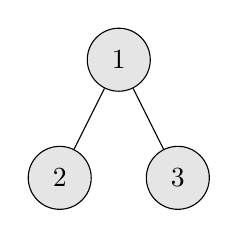
\begin{tikzpicture}
[every node/.style={draw, circle, minimum size=8mm, fill=gray!20!}]
\node{1}
child{node{2}}
child{node{3}};
\end{tikzpicture}
\end{figure}
\textbf{Output}: 2

\textbf{Explanation}: The longest consecutive path is $[1, 2]$ or $[2, 1]$.
 

\end{flushleft}

\paragraph{Example 2:}
\begin{flushleft}
\textbf{Input}:
\begin{figure}[H]
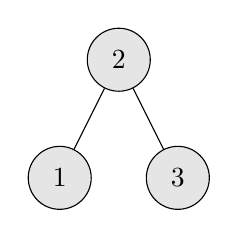
\begin{tikzpicture}
[every node/.style={draw, circle, minimum size=8mm, fill=gray!20!}]
\node{2}
child{node{1}}
child{node{3}};
\end{tikzpicture}
\end{figure}


\textbf{Output}: 3

\textbf{Explanation}: The longest consecutive path is $ [1, 2, 3] $ or $ [3, 2, 1] $.
\end{flushleft}
 

\paragraph{Note:} 
\begin{itemize}
\item All the values of tree nodes are in the range of $[-10^{7}, 10^{7}]$.
\end{itemize}

\subsection{Single Traversal}
\begin{itemize}
\item With every node, we associate two values named $x$ and $y$, where $x$ represents the length of the longest increment branch below the current node including itself, and $y$ represents the length of the longest decrement branch below the current node including itself.
\item We start off by assigning both $x$ and $y$ as 1 for the current node. This is because the node itself always forms a consecutive increasing as well as decreasing path of length 1.
\item Then, we obtain the length of the longest path for the left child of the current node recursively. Now, if the left child is less than the current node, it forms a decreasing sequence with the current node. Thus, the $y$ value for the current node is stored as the left child's $y$ value plus 1. But, if the left child is larger than the current node, it forms an increment sequence with the current node. Thus, we update the current node's $x$ value as left child's $x$ value plus 1.
\item Then, we do the same process with the right child as well. But, for obtaining the $x$ and $y$ value for the current node, we need to consider the maximum value out of the two values obtained from the left and the right child for both $x$ and $y$ since we need to consider the longest sequence possible.
\item After we've obtained the final updated values of $x$ and $y$ for a node, we update the length of the longest consecutive path found so far, $\ell$, as $\max(\ell, x+y-1)$.
\end{itemize}

\setcounter{lstlisting}{0}
\begin{lstlisting}[style=customc, caption={DFS}]
int longestConsecutive( TreeNode* root )
{
    if( !root )
    {
        return 0;
    }

    int x = 1;
    int y = 1;

    int best = 0;

    dfs( root, x, y, best );

    return best;
}

//x: the length of longest
//   incrementing sequence length below of current node
//   including current node
//y: the length of longest
//   decrementing sequence length blow of current node
//   inlcluding the current node
void dfs( TreeNode* node, int& x,  int &y, int& best )
{
    if( !node )
    {
        return;
    }

    int lx = 0;
    int ly = 0;

    if( node->left )
    {
        lx = 1;
        ly = 1;

        dfs( node->left, lx, ly, best );

        if( node->left->val == node->val - 1 )
        {
            //current node and left node
            //form a incrementing pair
            x = lx + 1;
        }
        else if( node->left->val == node->val + 1 )
        {
            //current node and left node
            //form a decrementing pair
            y = ly + 1;
        }
    }

    int rx = 0;
    int ry = 0;

    if( node->right )
    {
        rx = 1;
        ry = 1;

        dfs( node->right, rx, ry, best );

        if( node->right->val == node->val - 1 )
        {
            //current node and right node
            //form a incrementing pair
            //we need maximum one
            x = ( max )( x, rx + 1 );
        }
        else if( node->right->val == node->val + 1 )
        {
            //current node and right node
            //form a decrementing pair
            //we need maximum one
            y = ( max )( y, ry + 1 );
        }
    }

    best = ( max )( best, x + y - 1 );
}
\end{lstlisting}